\documentclass[11pt]{article}

% --- Page Layout (Standard Math / TCS) ---
\usepackage[utf8]{inputenc}
\usepackage[T1]{fontenc}
\usepackage[margin=1in]{geometry} % Sets 1-inch margins on all sides

% --- Core Math & Theorem Packages ---
\usepackage{amsmath, amssymb, amsthm}
\usepackage{mathtools} % Fixes minor amsmath quirks and adds extra tools

\usepackage{graphicx} % Required for inserting images

% --- Hyperlinks & Citations ---
\usepackage[colorlinks=true, citecolor=blue, linkcolor=blue, urlcolor=blue]{hyperref}
\usepackage[capitalise, noabbrev]{cleveref} % Lets you write \cref{thm:main} -> "Theorem 1"

\usepackage[dvipsnames]{xcolor} % Unlocks 68 richer named colors

% --- Caption Styling ---
\usepackage[
    font=small,          % Makes caption text slightly smaller than body text
    labelfont=bf,        % Makes "Figure 1:" bold (very clean in Math/TCS papers)
    margin=0.5in         % Adds 0.5-inch margin on BOTH left and right sides
]{caption}

% 1. Classic "Fast Forward / Rewind" (triangles touching tip-to-base)
\newcommand{\ffwd}{\ensuremath{\blacktriangleright\mkern-2.5mu\blacktriangleright}}
\newcommand{\rwnd}{\ensuremath{\blacktriangleleft\mkern-2.5mu\blacktriangleleft}}

% 2. Compact / Overlapping style (triangles slightly nested into each other)
\newcommand{\ffwdcompact}{\ensuremath{\blacktriangleright\mkern-5.5mu\blacktriangleright}}
\newcommand{\rwndcompact}{\ensuremath{\blacktriangleleft\mkern-5.5mu\blacktriangleleft}}

% Optional: Define your own custom hex or mixed colors
\definecolor{myorange}{HTML}{D98A00}     % Readable amber orange
\definecolor{mygreen}{rgb}{0.06, 0.62, 0.26} % Readable emerald green

% --- Theorem Environments ---
\newtheorem{theorem}{Theorem}[section]
\newtheorem{lemma}[theorem]{Lemma}
\newtheorem{corollary}[theorem]{Corollary}
\newtheorem{proposition}[theorem]{Proposition}

\theoremstyle{definition}
\newtheorem{definition}[theorem]{Definition}
\newtheorem{example}[theorem]{Example}

\theoremstyle{remark}
\newtheorem{remark}[theorem]{Remark}

% --- Custom Shortcuts ---
\newcommand{\R}{\mathbb{R}}
\newcommand{\N}{\mathbb{N}}
\newcommand{\Z}{\mathbb{Z}}
\newcommand{\E}{\mathbb{E}} % Expectation (very common in TCS)
\renewcommand{\Pr}{\mathbb{P}} % Probability

% --- Document Metadata ---
\title{BDO Worker Empire Solver}
%\author{i Mad}
\date{November 2026}

\begin{document}

\maketitle

\begin{abstract}
    We show that routing the BDO worker empire is an easy problem that can be solved in less than 2 seconds in pure JavaScript running on a browser.
\end{abstract}
    

\section{Introduction}
In Black Desert Online (BDO), we have a node system where we invest contribution points to connect nodes to nodes for various benefits, from sending workers to harvest the resources, to drop-rate bonus for grinding and selling price bonus for trading. The core question is the following:

\begin{quote}
    \emph{Given a set of pairs of nodes that we want to connect for resources and trading purposes, as well as a set of nodes that we want to connect to any town for grinding purposes. What is the least amount of CP that we need to invest?}
\end{quote}

This problem can be captured by the node-weighted Steiner forest problem for which we are given an undirected graph $G = (V, E)$, a weight function $w: V \to \R_{\ge 0}$, a set of terminal pairs $\{s_i, t_i\}$, $i = 1, \dots, k$ and the goal is to find a subset of vertices $U \subseteq V$ with minimum total weight $w(U) = \sum_{u \in U} w(u)$ such that for all $i \in [k]$, the pair $s_i$ and $t_i$ are in the same connected component of the induced subgraph $G[U]$.

It is easy to see that BDO worker empire can be formulated as a node-weighted Steiner forest problem when there are no nodes invested for grinding purposes: Let $G = (V, E)$ be the BDO node network with $w(u)$ equal to the CP needed for investing a node $u$, let $t_i$ be the resource or trading node that we want to take, and $s_i$ be the corresponding town or node where the assigned worker resides or trade goods were made.

When there are nodes that are invested for grinding, we can still model it as a node-weighted Steiner forest problem by introducing a star gadget for each grind node: for each $t'_j$ that can be connected to any town, introduce a star graph with weight 0 central vertex $s'_j$ and a set of leaves $x_{j, i}$, $i = 1, \dots, N$ where $N$ is the number of towns, each with weight $W$ for a sufficiently large $W$ (say, take $W = 1 + \sum_{v \in V} w(v)$), then for each $i$, connect $x_{j, i}$ to a distinct town node and add a terminal pair $\{s_j', t_j'\}$. The heavy weight on $x_{j, i}$ prevents a free target from selecting more than one such bridge to enable a highway between towns.


Node-weighted Steiner forest generalizes the classic Steiner tree problem. The decision version of the Steiner tree problem is one of Karp's 21 NP-complete problems, which makes the node-weighted forest version NP-hard in general. However, for the tree version where there is a common intersection over all the terminal pairs, exact fixed-parameter tractable (FPT) algorithms and approximation schemes are known for various classes of graphs. There are also practical integer-linear programming based solvers and SCIP-Jack is one of the most efficient.

In this note, we show that the basic dynamic programming on tree decomposition works well for the BDO worker empire problem.\\

\noindent
\textbf{On AI usage}. Gemini was used to fix the typos and help improving the presentation in Section \ref{solve} as well as generating Figure \ref{fig:merge_partition}. On the coding side, Gemini was heavily used to help understanding how Vue, Pinia and JavaScript work as well as implementing most of the features (especially all the css style and html elements). Gemini 3.5 or 3.8 on Low thinking level was the main one used throughout the project until close to the end when version 4 Neon was available I switched to that on High setting for the final implementation of the DP algorithm after a couple of inefficient or buggy attempts from lower setting and it pretty much just one-shot the implementation with $3,000+$ lines of code. Prior to this, I never even used GitHub and never wrote any JavaScript or website before so this work would not be possible without the assistance from it.



\section{Notation, terminology and code related elements}
Throughout this note and the visualization components in the solver, we denote $G = (V, E)$ the BDO node network (undirected) graph. We may call an element in $V$ either a node or a vertex. The node weight $w(u)$ or $CP(u)$ is the contribution points (CP) required for investing the node $u \in V$.

\begin{enumerate}
    \item[$\bullet$] \textbf{Plantzone nodes}. These are nodes that generate resources and we can assign workers to. They are nodes with key \texttt{pzk} such that \texttt{gameStore.isPlantzone(pzk)} is true. Alternatively, they are nodes in \texttt{plantzone.json} where \texttt{kind} is not equal to 10, 12 or 13. There are currently 370 of such nodes. Plantzone nodes have degree 1 in $G$ and we call their neighbors their \textbf{parents}.

    \item[$\bullet$] \textbf{Towns}. Towns are set to be nodes with CP 0 and \texttt{kind} 1 or 2 according to \texttt{gameStore.nodes}. There are 35 nodes that satisfy this condition and are considered to be towns. Note that it is not the best definition as pointed out in a comment by Shrddr inside \texttt{game.js}.

    \item[$\bullet$] \textbf{Targets and sources}. Targets are the nodes that we are going to take and sources are the corresponding nodes that the target connects to. In terms of BDO worker empire, targets are either the nodes that we pick for the resources or selling trade goods and the sources are the nodes where the assigned worker resides or the origin of the trade goods. In Steiner type problem terminology, a target and the corresponding source is a terminal pair. A target is \textbf{\emph{free}} if it suffices to connect it to any town, i.e., a node that we take for grinding droprate in BDO.
\end{enumerate}

Without any preprocessing, at the current moment the BDO node network has 370 plantzone nodes, 35 towns (21 kind 1 and 14 kind 2, there are more kind 1 nodes but some of them cost CP), and 534 possible free targets. The entire graph has 1006 nodes and 1122 edges.

The graph processing panel (\texttt{GraphProcessingPanel.vue}) is the main Vue component we added on top of Shrddr's workerman. It contains all the instance generation and management (Section \ref{instance}), preprocessing (Section \ref{reduce}) and the solver (Section \ref{solve}) as well as their visualization. A more detailed list of changes vs Shrddr's original version can be found in Appendix \ref{change}.


\section{Instance generation}
\label{instance}
There are three slider bars on the \texttt{INSTANCE} tab and each bar comes with a forward/backward button where you can trigger fast forward/rewind by holding the mouse click on them longer. When the icons are animated (controlled by the top right button next to \texttt{?}), all the changes are applied continuously while dragging the slider bar. When the die icon is on, the given seed is in use and the instance is generated deterministically using that seed. There are two modes for choosing the set of targets and two modes for assigning the source towns:

\begin{enumerate}
    \item[$\bullet$] Target plantzone selection ($n \in \{1, 2, \dots, 370\}$)

    \begin{enumerate}
        \item Permute the plantzone nodes and select the first $n$. The random permutation is generated using Fisher-Yates shuffle with the given seed (same for the following when a random permutation is involved).

        \item Select the $n$ highest profit plantzone nodes according to \texttt{gameStore.allPzProfit}. No randomness is involved.
    \end{enumerate}

    \item[$\bullet$] Source town selection ($k \in \{1, 2, \dots, 30\}$ / $r \in \{1, 1.02, 1.04, \dots, 1.58\}$)

    \begin{enumerate}
        \item For each target, select a uniform random town among the closest $k$ towns (more precisely, up to $k$ highest profit towns if the worker there was sent).

        \item A matching strategy that is somewhat similar to stable marriage (hence why the icon is a pair of rings). Like stable marriage, each town has its own preference list over the targets which is ranked by the profit of sending a worker there (in decreasing order of profit). Towns are permuted randomly first, then we proceed in rounds. In each round, the towns propose to their next most preferred target plantzone one by one according to the random order on the towns. If the target plantzone node is not engaged, it accepts the proposal. If the target is already engaged, we check if the new proposal is $r$ times better than the current one (in terms of profit). It breaks up with the current engaged town and accept the proposal from the new one if and only if the new proposal is $r$ times better. When $r = 1$ it reduces to stable marriage (when lodging caps are not considered) and it is the same as closest $k$ town matching with $k = 1$.
    \end{enumerate}

    \item[$\bullet$] Free target non-plantzone selection ($m \in \{1, 2, \dots, 534\})$

    \begin{enumerate}
        \item[$\circ$] Select the first $m$ non-plantzone nodes over a random permutation.
    \end{enumerate}
\end{enumerate}


Whenever a target is changed on the map, either by clicking the node while quick select is activated or choosing the town in the bottom left tab, the change will disable the random instance and the resulting instance would be saved as a custom instance. One can also upload an instance encoded in a \texttt{json} file. To switch between these instances, you can hold the refresh button next to the die button and a dropdown tab will appear and you can choose between those instances. Also note that there is a batch seed generation panel in that tab. Clicking the refresh button will generate a new seed and a new random instance will be constructed.

A mini \texttt{REDUCE} and \texttt{SOLVE} tab are available as drop-down tabs, which allow you to view any reduced instance and run the solver (and visualize the solution) directly.


\section{Graph preprocessing}
\label{reduce}
On the \texttt{REDUCE} tab, we apply a couple basic preprocessing steps iteratively to shrink the size of the instance. The result of each step is logged into an array \texttt{graphStore.reducedGraph} and shown on the map in real-time. You can either drag the slide bar, press the $\blacktriangleleft$ and $\blacktriangleright$ buttons or even press the directional keys $\leftarrow$ and $\rightarrow$ on the keyboard to go to the next/previous graph (fast forward/rewind will be triggered by holding it longer). There are also \rwndcompact \ and \ffwdcompact \ buttons that will get all the way to the end of a stage (see below for what it means by a "stage"). The whole preprocessing procedure is as follows:


\begin{enumerate}
    \item[$\bullet$] \texttt{CLEANUP} If a plantzone node is not a target, we can simply remove it. If it is a target, then we must select its parent too so one can select its parent as a target, add its CP to its parent and then remove it. Investment bank nodes are also removed in this step. It immediately cut down $400+$ nodes (and edges as each of them has degree 1) from the graph.

    \item[$\bullet$] Repeat the following stages until no further changes can be made. For each stage, repeat until no more changes can be made before moving on to the next.

    \begin{enumerate}
        \item[1.] \texttt{DEGREE1\_PRUNE}. Removing degree 1 non-town nodes. If a target has degree 1, then in order to get there its neighbor must be taken too. Thus, one can remove the degree 1 target and make its neighbor to be the target (with the same source town), add its CP to its neighbor and remove it. If a non-target non-town has degree 1, there is no point in taking this and hence can just be removed.

        \item[2.] \texttt{DEGREE2\_CONTRACT}. Contracting adjacent degree 2 non-target non-town nodes. If two adjacent non-target non-town nodes both have degree 2, then in the optimal solution we must take either none or both. Since for contradiction suppose we only take one of them in the optimal solution, then the taken one would have degree 1 and since it is not a target and not a town and hence has positive CP, we can remove it from the solution and it still satisfies the connectivity requirement for all free targets and target-source pairs. Contradicting with the assumption that the solution is optimal.

        \item[3.] \texttt{TARGET\_MERGE}. Merging adjacent targets. If two targets $u$ and $v$ are adjacent to each other, then one can treat them as a single target with source towns between the union of the two original sources. A bit more formally, any feasible solution in the reduced graph has a corresponding feasible solution in the original graph with the same cost by splitting $u$ and $v$ (and vice versa by merging $u$ and $v$).

        \item[4.] \texttt{REDUNDANT\_NODE}. Removing redundant degree 2 non-target non-town nodes. Let $u$ be a degree 2 non-target node with neighbors $v$ and $w$. If there is a path from $v$ to $w$ without using $u$ and has node weighted cost (excluding the cost of $v$ and $w$) at most the cost of $u$, then $u$ can be removed because if $u$ was in the optimal solution one can remove $u$ and take the alternative path from $v$ to $w$ instead.

        \item[5.] \texttt{TOWN\_REDIRECT}. Regrouping the targets. If there is a node that needs to be connected to both town $a$ and $b$, then $a$ and $b$ must be in the same connected component in any feasible solution. Thus, one can treat $b$ as a regular node (demoting its town status) and add it as a target with source town $a$. Then redirect all the targets being associated with $b$ to $a$ instead. It is straightforward to check that the two instances have the same set of feasible solutions with the same cost.
    \end{enumerate}
\end{enumerate}

After these preprocessing steps, a typical random instance has around $\sim 260$ nodes and $\sim 340$ edges left. The number of degree 2 and 3 non-target non-town nodes is $\sim 100$ and $\sim 70$ respectively (and a few for degree $4+$). Note that these are the only decisions we need to make as other nodes must be in the solution already. It shows the true scale of the problem.

The original graph without any targets has treewidth at most 9. And in the vast majority of the cases, the treewidth drops to 7 or less after these basic preprocessing steps, which immediately implies the tree version of the problem is easily solvable in real-time using basic dynamic programming on the tree decomposition. 



\section{Solver}
\label{solve}

In the \texttt{SOLVE} tab of the graph processing panel, a \texttt{svg} plot of the tree is shown and in that view window you can scroll to zoom in/out, drag to move, and click to select a tree node (the node is a bit small so could be hard to select). You can also navigate through the tree by clicking the buttons: $\blacktriangle$ for moving up to the parent; $\blacktriangleleft$ for moving to the left sibling; $\blacktriangleright$ for moving to the right sibling and $\blacktriangledown$ for moving to the second child (from left to right, or the only child if there is only one). You can also use the directional keys on the keyboard and they function the same as clicking those buttons, except that if you press $\downarrow$ while holding $\leftarrow$ and $\rightarrow$ you will move to the left-most and right-most child respectively. Both the tree \texttt{svg} plot window and the bag (tree node) information tabs are drop-down tabs that we can hide.


\subsection{Tree decomposition}
Roughly speaking, a tree decomposition maintains a set of ``snapshots'' of the graph in an acyclic way where each ``snapshot'' is, in a sense, a cut that separates the graph. These ``snapshots'' are the nodes in the tree decomposition and they are called the \textbf{bags}. Each bag is a subset of vertices in the original graph. We will demonstrate what a tree decomposition is visually. 

When you are on the \texttt{SOLVE} tab of the graph processing panel with the \texttt{svg} tree plot on, you can hover over any node or edge on the map. In both \texttt{FULL} and \texttt{JOIN} tabs of the plot, when you hover over a node in the map, all the bags containing that node will be highlighted. If you are on the \texttt{FULL} tab the bag(s) containing both endpoints of that edge will be highlighted and if you are on the \texttt{JOIN} tab (which is a compact binary version of the \texttt{FULL} tree) the tree edge that corresponds to the endpoint of that edge will be highlighted.

Formally, a tree decomposition is a tree over the bags that satisfies the following properties (which you should check each of them visually by hovering over the nodes and edges in the map):

\begin{enumerate}
    \item Every node in the original graph is contained in some bag.

    \item For every edge in the original graph, there is a bag that contains both endpoints of that edge.

    \item (Running intersection property) For every node in the original graph, all the bags containing that node are connected (i.e., forming a subtree).
\end{enumerate}


Property 3 is crucial for doing leaf-to-root dynamic programming (DP). This property implies an important structure---When we walk from a leaf to the root and keep track of what nodes appear in the bags along the way. A node that leaves the bag is gone forever and we will not see that again in any bags above.


Another crucial property follows from properties 2 and 3 together---every bag in the tree decomposition cuts the graph into pieces where the nodes in the bag are the only communication interface between those pieces (it is not quite accurate as some of the pieces can be empty). This property can be checked visually on the map. When you click a node on the \texttt{svg} tree plot, there will be a yellow $\times$ drawn on top of the nodes contained in that bag.

Consider the \texttt{JOIN} tree as it is a binary tree (which simplifies the following explanations). Suppose the tree node we clicked was $u$ and $B_u$ is the bag. Let $l$ and $r$ be the left and right children of $u$ in the tree. Then on the map, you will see a bunch of $\times$ icons highlighting $B_u$, and colored edge highlights that partition the remaining graph into up to 3 regions (the following notation is also used in the legend on the map): 

\begin{enumerate}
    \item \textbf{$B_u$ marked by the icon $\times$}. Nodes of the original graph that appears in $B_u$.

    \item \textbf{$T_l \setminus B_u$ marked by green edge highlight}. Nodes of the original graph that appear in some bags in the subtree rooted at $l$ but not $B_u$.

    \item \textbf{$T_r \setminus B_u$ marked by purple edge highlight}. Nodes of the original graph that appear in some bags in the subtree rooted at $r$ but not $B_u$.

    \item \textbf{$V \setminus T_u$ marked by blue edge highlight} All the remaining nodes from the original graph.
\end{enumerate}

Note that depending on which node you clicked on, $T_l \setminus B_u$ and $T_r \setminus B_u$ can be empty. However, when they are not, you will see that going from one region to another must pass through the nodes in the bag (the $\times$ nodes on the map). In other words, $B_u$ is a \textit{vertex separator} of the graph.


\begin{figure}[htbp]
    \centering
    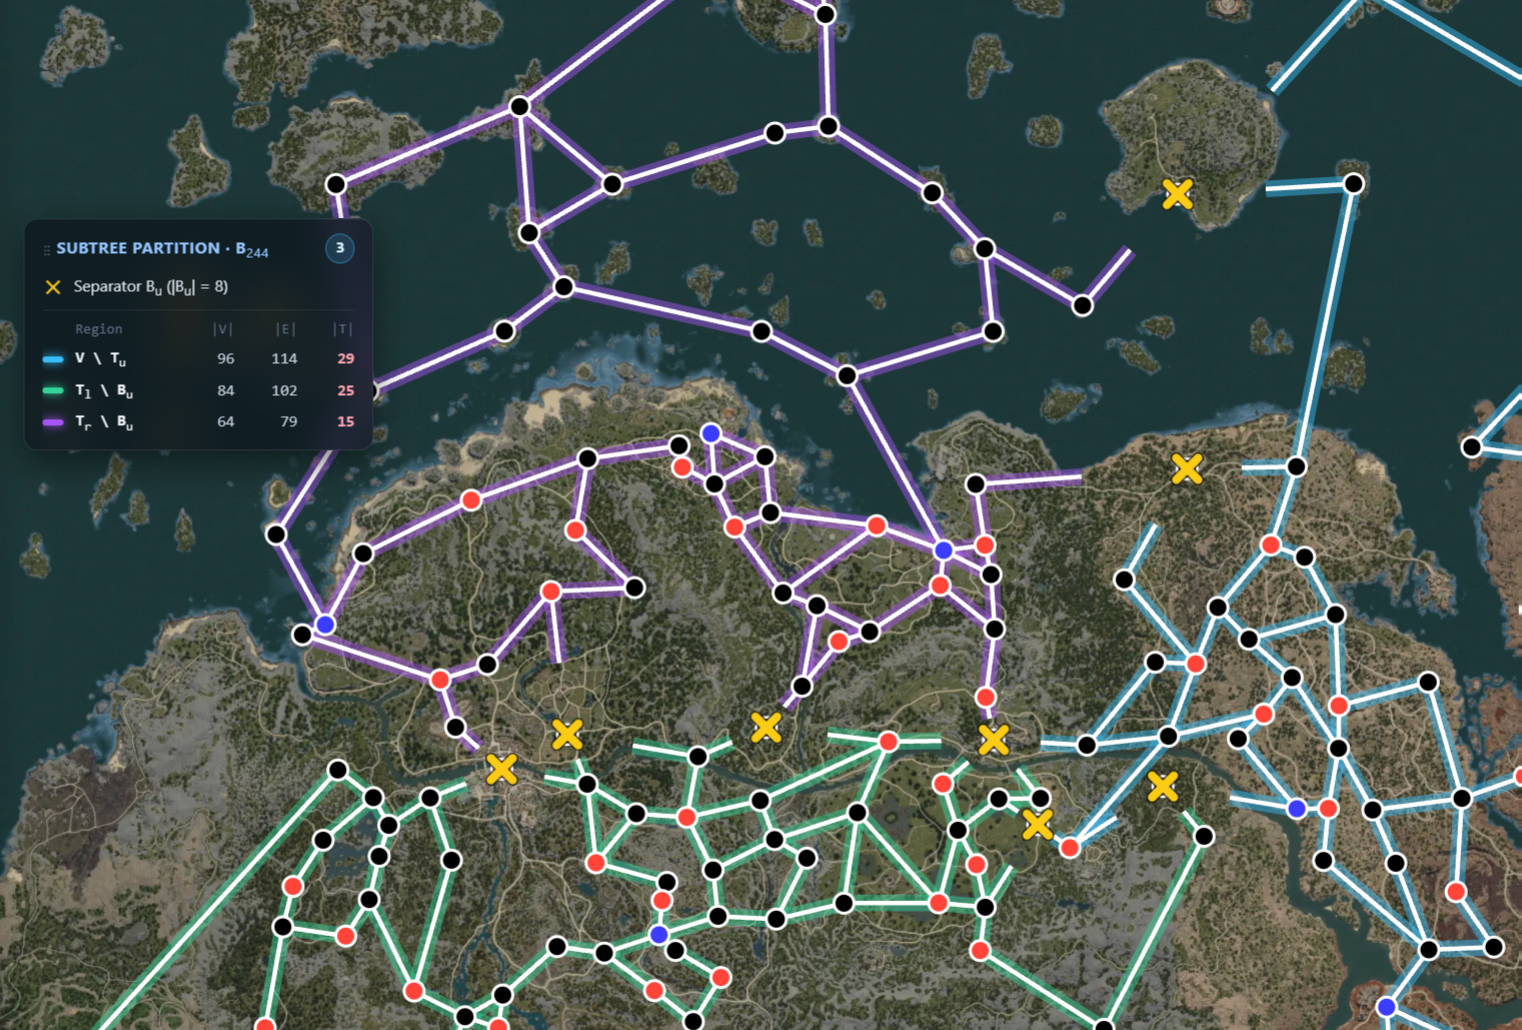
\includegraphics[width=0.7\textwidth]{join.png}
    \caption{Partitioning the preprocessed graph. The nodes in the bag $B_u$ (of size 8) are marked by yellow $\times$ icons. Three colored regions are shown: green region for nodes that appear only in the left subtree ($T_l \setminus B_u$); purple region for nodes that appear only in the right subtree $T_r \setminus B_u$ and blue region for the remaining nodes. It shows visually the property that in order to go from one region to another, one must pass through some $\times$ (the nodes from the bag $B_u$).}
    \label{fig:join}
\end{figure}


(Skip to the next subsection if you are convinced by the visualization that each bag indeed separates the graph into those regions unless you want to see how to show that formally.)

In fact, it is not immediately clear why the definition above even forms a partition on the nodes as $T_l \setminus B_u$ and $T_r \setminus B_u$ could have non-empty intersections. Now we show that they cannot share any vertices by using property 3 (the running intersection property): Suppose there is a common node $x$ from the original graph that appears in both $T_l \setminus B_u$ (contained in some bags in the left subtree but not $B_u$, the green region in Figure \ref{fig:join}) and $T_r \setminus B_u$ (contained in some bags in the right subtree but not $B_u$, the purple region in Figure \ref{fig:join}). Let $v$ and $w$ be the corresponding tree nodes whose bags contain $x$. Then property 3 says that $x$ appears in \textbf{all} bags along the unique path between $v$ and $w$, which includes $u$ in particular. Thus, $x \in B_u$, which is a contradiction.

With property 2, the argument above also implies the property that each bag in the tree decomposition forms a vertex separator that cuts the graph into those regions (provided that at least two regions are non-empty). Property 2 asserts that for every edge $\{x, y\}$ in the original graph, there is a node $v$ in the tree with bag $B_v$ that contains both endpoints. Now, suppose there is an edge $\{x, y\}$ where $x$ in $T_l \setminus B_u$ (the green region) and $y$ in (i) $T_r \setminus B_u$ (the purple region) or (ii) $V \setminus T_u$ (the blue region). In either case, $y$ is not in any bag inside the left subtree, which means that the tree node $v$ with bag $B_v$ that contains both $x$ and $y$ is not located inside the left subtree. However, by property 3 $x$ appears in all bags along the path from a node inside the left subtree to $v$. Since this path includes the tree node $u$, we have the contradiction $x \in B_u$ again.


\subsection{Dynamic programming for a single group}
Recall that in the node-weighted Steiner forest problem we are given a set of terminal pairs $\{s_i, t_i\}$. For the BDO worker empire, $t_i$ corresponds to a plantzone (or trade) node and $s_i$ corresponds to the town where the worker resides (or the trade origin). Even when trading pairs are included, the number of distinct sources is small. Considering only the fixed terminal pairs, we partition the mandatory vertices into pairwise-disjoint \textbf{groups} given by the connected components of the demand graph (two terminals belong to the same group whenever they share a source town, or are linked transitively through shared endpoints). Free targets do not belong to a fixed group; we defer them to Section~\ref{sec:multi_group}.

While the Steiner tree problem admits a standard DP on a tree decomposition running in time $f(k)\cdot |V|$ where $k$ is the maximum bag size (as small as treewidth plus $1$), the Steiner forest problem remains NP-hard even on graphs of treewidth $3$. However, because one can reduce a multi-group instance to a collection of Steiner trees by guessing which groups merge into the same connected components in an optimal solution, the problem is fixed-parameter tractable in the treewidth and the number of groups $g$.

We first consider the single-group case ($g = 1$), where all targets share a common source town---for example, sending Calpheon workers to every chosen plantzone. This is the node-weighted Steiner \textit{tree} problem. We describe the textbook bottom-up DP on a tree decomposition here, and extend it to multiple groups and free targets in the next subsection.

Following the formal definition of a tree decomposition in the previous subsection, two structural properties make bottom-up DP work:
\begin{enumerate}
    \item[(a)] Along any leaf-to-root path in the tree, once a vertex leaves the bag, it never reappears.
    \item[(b)] The vertices in a bag $B_u$ form the only ``communication interface'' between the regions separated by $B_u$.
\end{enumerate}

Focus first on~(b). Recall Figure~\ref{fig:join}, where a bag $B_u$ separates the graph into regions that can only interact through $B_u$. Suppose for simplicity that $u$ is a root join node with left child $l$ and right child $r$, so the entire graph is covered by the two subtrees $T_l$ (the green region together with $B_u$) and $T_r$ (the purple region together with $B_u$), with $T_l \cap T_r = B_u$. Once we fix what happens on $B_u$, the two subproblems on $T_l$ and $T_r$ decouple completely.

Let $U^* \subseteq V$ be an optimal solution to the Steiner tree problem, and let $A = B_u \cap U^*$ be the subset of bag vertices selected by $U^*$. Define $U_l^* = T_l \cap U^*$ and $U_r^* = T_r \cap U^*$, so that $U^* = U_l^* \cup U_r^*$ and $U_l^* \cap U_r^* = A$. In general, the induced subgraphs $G[U_l^*]$ and $G[U_r^*]$ consist of collections of connected components satisfying:
\begin{enumerate}
    \item[(i)] Every target in $T_l$ (resp.\ $T_r$) is included in $U_l^*$ (resp.\ $U_r^*$), and every connected component containing a target must intersect $A$---otherwise that component would be disconnected from the rest of the graph (except in the boundary case where $A = \emptyset$ and \emph{all} targets of the entire instance lie inside $T_l \setminus B_u$, or all inside $T_r \setminus B_u$).
    \item[(ii)] Every vertex in $A$ belongs to some connected component of $G[U_l^*]$ (resp.\ $G[U_r^*]$). Thus, the connected components of $G[U_l^*]$ and $G[U_r^*]$ each induce a partition of $A$ (not necessarily the same partition).
    \item[(iii)] Among all subsets of $T_l$ (resp.\ $T_r$) intersecting $B_u$ in $A$ that satisfy~(i) and induce the same partition on $A$ in~(ii), the subset $U_l^*$ (resp.\ $U_r^*$) has minimum total vertex weight.
\end{enumerate}

Properties~(i) and~(ii) follow directly from feasibility. To see why~(iii) holds, observe that combining the induced partitions of $A$ from $T_l$ and $T_r$ determines the resulting connectivity on $A$ purely from those two partitions. For illustration, consider Figure~\ref{fig:merge_partition}, where $A = \{a_1, a_2, a_3, a_4\}$. In the green region ($T_l$), the connected components induce the partition $\{\{a_1, a_2\},\, \{a_3\},\, \{a_4\}\}$. In the purple region ($T_r$), the connected components induce $\{\{a_1\},\, \{a_2, a_3\},\, \{a_4\}\}$, where $P_2 = \{a_2, a_3\}$ contains no targets and serves purely as a Steiner bridge. Merging both sides connects $G_1$, $P_2$, and $G_2$ into a single component, yielding the coarser partition $\{\{a_1, a_2, a_3\},\, \{a_4\}\}$ on $A$.

\begin{figure}[htbp]
    \centering
    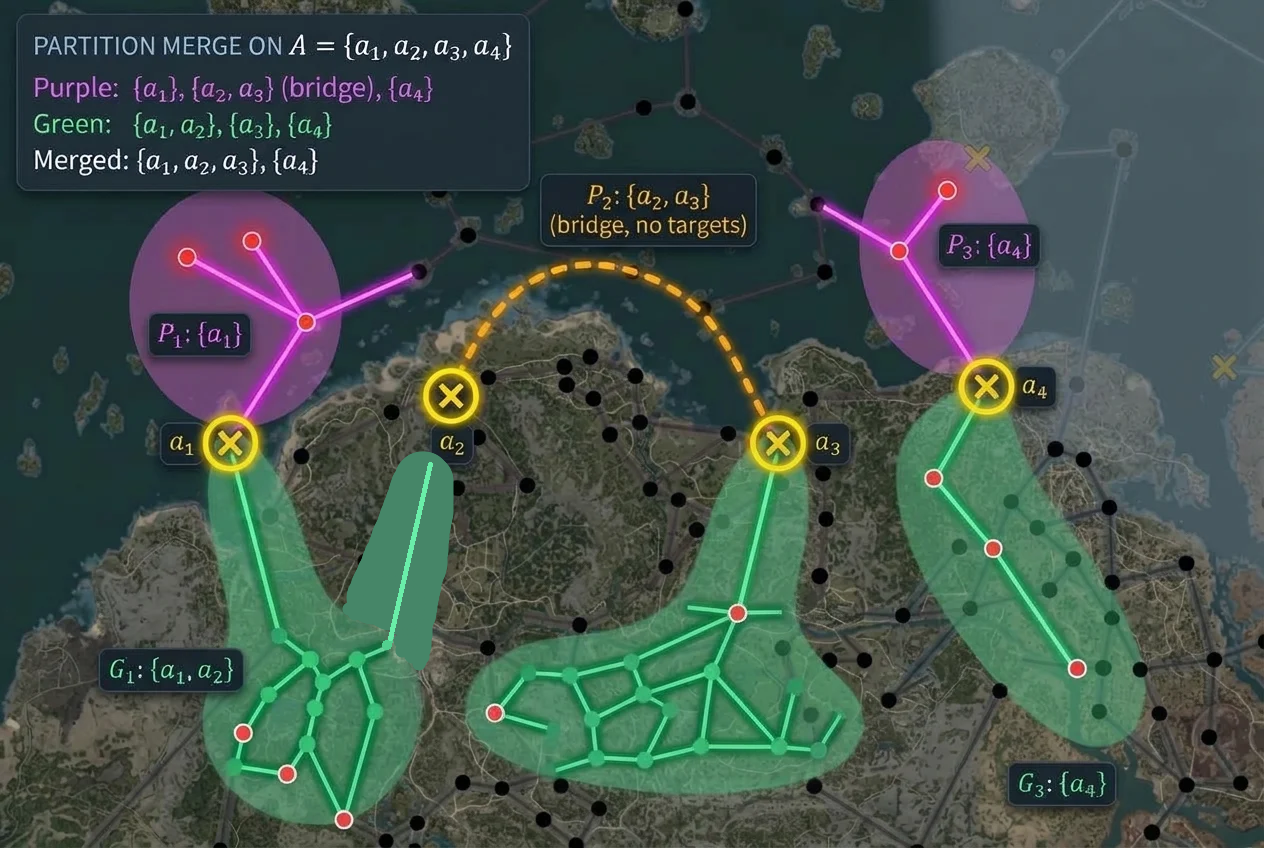
\includegraphics[width=0.75\textwidth]{merge_partition.png}
    \caption{Merging connectivity partitions on an active separator subset $A = \{a_1, a_2, a_3, a_4\} \subseteq B_u$ (with the blue region $V \setminus T_u$ dimmed). The purple region induces $\{\{a_1\}, \{a_2, a_3\}, \{a_4\}\}$, where $P_2 = \{a_2, a_3\}$ contains no targets and acts purely as a bridge. The green region induces $\{\{a_1, a_2\}, \{a_3\}, \{a_4\}\}$. Combining both regions fuses $G_1$, $P_2$, and $G_2$, producing the merged partition $\{\{a_1, a_2, a_3\}, \{a_4\}\}$ on $A$.}
    \label{fig:merge_partition}
\end{figure}

Because the merged connectivity depends only on the two partitions of $A$---not on the internal routing inside $T_l \setminus B_u$ or $T_r \setminus B_u$---if $U_l^*$ were not a minimum-weight realization for its induced partition, replacing $U_l^*$ with a lighter one would strictly reduce $w(U^*)$, contradicting optimality. Moreover, because the vertices in $A$ are counted in both $U_l^*$ and $U_r^*$, the total weight of a merged solution is
\[
    w(U_l^* \cup U_r^*) = w(U_l^*) + w(U_r^*) - w(A).
\]
At the root, taking the minimum over all pairs of compatible child states whose merged partition consists of a single block (containing all vertices of $A$) recovers the exact Steiner tree optimum.

To compute the tables bottom-up, each bag $B_u$ stores, for every reachable subset $A \subseteq B_u$ and every partition $\pi$ of $A$, the minimum weight of a partial solution in $T_u$ that covers all targets in $T_u$ and induces $\pi$ on $A$. Choosing $A \subseteq B_u$ together with a partition of $A$ is equivalent to partitioning $B_u \cup \{\bot\}$ (where unselected vertices sit in the block of $\bot$), so the worst-case number of states for a bag of size $k$ is the Bell number $B_{k+1}$. In our preprocessed instances, the largest bag typically has size $8$ (treewidth $7$, at most $B_9 = 21{,}147$ states) or size $9$ (treewidth $8$, at most $B_{10} = 115{,}975$ states). In practice, far fewer states arise because planarity rules out crossing partitions, and upper/lower bound pruning eliminates almost all suboptimal states early.

Finally, as we walk leaf-to-root along the tree decomposition, vertices enter and leave the bags: when a vertex enters a bag it is \textbf{introduced}, and when it leaves a bag it is \textbf{forgotten}. In the \texttt{FULL} tree, adjacent bags differ by a few introduce/forget steps; in the contracted \texttt{JOIN} tree, an entire chain of introduce and forget steps between a child bag $B_l$ and its parent bag $B_u$ is compressed into a single edge. Before performing the join at $u$, we lift each child's DP table along its contracted edge to match $B_u$:
\begin{enumerate}
    \item[$\bullet$] \textbf{Forget.} When a vertex leaves the bag, by property~(a) it will never reappear. If forgetting vertices causes an entire connected component to disappear from the bag, we check whether that component contains any targets:
    \begin{enumerate}
        \item If it contains no targets, it is a disconnected Steiner-only component and the state is discarded.
        \item If it contains targets, the state is discarded whenever any target exists outside that component (either in another block of the current bag or in $V \setminus T_u$). Only if \emph{no} targets exist elsewhere can that single forgotten component be marked as a completed solution.
    \end{enumerate}
    \item[$\bullet$] \textbf{Introduce.} When a new vertex $v$ enters the bag, we branch on excluding $v$ (disallowed if $v$ is a mandatory target) or including $v$ in $A$ (adding $w(v)$ to the cost and merging all existing blocks of $A$ adjacent to $v$).
\end{enumerate}
Once both child tables have been lifted to $B_u$, we join every pair of left and right states sharing the same active subset $A$, merge their partitions via union-find, subtract $w(A)$, and keep the minimum cost per resulting state. Visually, moving up one step in the \texttt{JOIN} tree plot shows the green and purple regions combining into a single child region of the parent, repeating until the root is reached.


\subsection{Dynamic programming for multiple groups}
\label{sec:multi_group}
Extending the single-group DP to $g$ pairwise-disjoint fixed terminal groups is straightforward. In addition to tracking the active subset $A \subseteq B_u$ and its partition into blocks $c \in \{1, \dots, m\}$, each block $c$ stores two pieces of metadata:
\begin{enumerate}
    \item[$\bullet$] \textbf{Active group bitmask} ($g$ bits): which fixed terminal groups intersect block $c$ and are not yet fully resolved. A group's bit is cleared immediately once all of its terminals have been seen inside $T_u$ and lie within a single block of $A$ (since its connectivity requirement is already satisfied).
    \item[$\bullet$] \textbf{Terminal presence bit} ($1$ bit): whether block $c$ contains at least one mandatory vertex. This prevents a forgotten Steiner-only component from surviving in the DP table.
\end{enumerate}

When a block disappears during a forget step, the state is valid if and only if the forgotten block has no active group bits set (so no fixed group is split across the cut) and has its terminal presence bit set (so no useless Steiner-only component is left behind). At a join node, merging two blocks simply takes the bitwise OR of their active group bitmasks and terminal presence bits, and then clears any group bit that has no terminals remaining in $V \setminus T_u$ and now appears in only one block of $A$.

In the worst case, attaching a $g$-bit group mask to each block multiplies the state space by up to $2^g$ per block. In practice, states are generated dynamically only when reachable, and because BDO instances are sparse and planar, the number of states that actually arise is tiny compared to the theoretical bound; in our experiments, $1{,}024$ states per bag is usually already sufficient to find an optimal solution.

\paragraph{Handling free targets.}
Free targets (nodes invested for grinding drop-rate) do not need to connect to each other, nor necessarily to another fixed target group---each free target only needs to connect to \emph{any} town, including towns with no assigned workers. Treating each of the $m$ free targets as its own group would add $m$ extra bits per block. Instead, we handle all free targets simultaneously using just \textbf{two extra bits per partition block}:
\begin{enumerate}
    \item[$\bullet$] \texttt{hasTown} ($1$ bit): set to $1$ if the block already contains at least one town vertex.
    \item[$\bullet$] \texttt{needsTown} ($1$ bit): set to $1$ if the block contains at least one free target and \emph{no} town yet.
\end{enumerate}
Whenever a block acquires a town---either when a town vertex is introduced into it, or when it merges with a block having $\texttt{hasTown} = 1$ during a join---its \texttt{needsTown} bit is immediately cleared to $0$. Tracking both bits is essential across joins: if a block in the left subtree holds a town ($\texttt{hasTown} = 1$, $\texttt{needsTown} = 0$) and a block in the right subtree holds an unsatisfied free target ($\texttt{hasTown} = 0$, $\texttt{needsTown} = 1$), merging them immediately resolves the free target ($\texttt{hasTown} = 1$, $\texttt{needsTown} = 0$). During a forget step, any block leaving the bag with $\texttt{needsTown} = 1$ corresponds to a stranded free target and the state is discarded; similarly, at the root, all surviving blocks must satisfy $\texttt{needsTown} = 0$.


\subsection{State management}
\label{sec:state_mgmt}
Although the worst-case DP table size grows rapidly with treewidth and $g$, BDO instances exhibit strong spatial locality. When targets are assigned to nearby towns, each group's terminals lie close together in the tree decomposition and its active bit is cleared quickly; when targets are assigned to distant towns, their paths collide across the sparse planar map, collapsing groups early during preprocessing (Section~\ref{reduce}).

To guarantee exactness within browser memory limits, we combine exact per-partition dominance cleanup with tight primal upper bounds and strictly admissible dual lower bounds on the unprocessed outside graph $O = V \setminus T_u$ (the blue region in Figure~\ref{fig:join}):

\begin{enumerate}
    \item[$\bullet$] \textbf{Upper bound.} Before running the DP, a fast greedy heuristic produces a feasible Steiner forest in under $10\text{ ms}$. Across six orderings of the fixed groups (descending size, ascending size, natural, reverse, and two deterministic shuffles), it starts with all mandatory vertices selected, iteratively runs multi-source Dijkstra from the smallest terminal component of each group (charging $0$ for already-selected vertices) until all groups are connected, attaches any remaining unsatisfied free targets to their cheapest reachable town, and finally scans chosen Steiner vertices in descending weight order, deleting any vertex whose removal preserves feasibility. When stronger bounds are needed before the exact pass, the solver runs a cascading schedule of width-capped beam DP passes and partition-guided exact single-tree refinements (\texttt{GREEDY} $\to$ \texttt{HEUR 1K} $\to$ \texttt{POLISH} $\to$ \texttt{HEUR 4K} $\to$ \texttt{HEUR 16K} $\to$ \texttt{EXACT}) to tighten the incumbent upper bound $\mathrm{UB}$.

    \item[$\bullet$] \textbf{Lower bound.} For each DP step with outside region $O = V \setminus T_u$, we first compute the exact total weight $L_{\mathrm{mand}}$ of all mandatory vertices in $O$, and set their weights to $0$ inside $O$ so that mandatory costs are never double-counted with Steiner costs. We then compute an admissible two-layer lower bound on the Steiner vertices of $O$:
    \begin{enumerate}
        \item \emph{Contracted-interface dual ascent (partition-independent).} For each active bag subset $A \subseteq B_u$, we contract $A$ into a single zero-weight super-vertex $u^*$ (inheriting the union of active groups seen in $T_u$) and run node-weighted primal-dual moat growth (as in Demaine--Hajiaghayi--Klein, without reverse deletion) on $O \cup \{u^*\}$. Starting from the connected components of $u^*$ and zero-weight vertices in $O$, all active components grow simultaneously until a boundary Steiner vertex $v \in O$ becomes tight, yielding a dual lower bound $\mathrm{dualLB}(A)$ together with non-negative \textbf{residual weights} $\mathrm{resW}[v] \le w(v)$ for every Steiner vertex $v \in O$. Because contracting $A$ only relaxes connectivity, $\mathrm{dualLB}(A)$ is valid for every partition of $A$ and is cached once per subset $A$.
        \item \emph{Residual split-group bound (partition-specific).} Contracting $A$ ignores the cost of joining distinct blocks of $A$ that share a split group. Using strictly the leftover residual weights $\mathrm{resW}[v]$, we compute shortest outside distances between pairs of vertices in $A$. For any DP state with a group split across multiple blocks, every split block $c$ must connect to some vertex in $A \setminus c$ through $O$, incurring residual cost at least its minimum exit distance $\mathrm{minExit}(c)$. Setting $\mathrm{extraLB} = \max_{c \text{ split}} \mathrm{minExit}(c)$ avoids double-counting shared exit paths. By weak duality, every outside Steiner completion $S_O \subseteq O$ satisfies
        \[
            \sum_{v \in S_O} w(v) = \sum_{v \in S_O}\bigl(w(v) - \mathrm{resW}[v]\bigr) + \sum_{v \in S_O} \mathrm{resW}[v] \;\ge\; \mathrm{dualLB}(A) + \mathrm{extraLB},
        \]
        so $L_{\mathrm{mand}} + \mathrm{dualLB}(A) + \mathrm{extraLB}$ is a strictly admissible lower bound with zero double-counting.
    \end{enumerate}

    \item[$\bullet$] \textbf{Pruning and optimality certification.} Lower-bound pruning is applied at every introduce, forget, and join step (inside joins, left and right state buckets for each subset $A$ are sorted by cost so pairs exceeding the threshold break out of the loop early). In addition, within each partition bucket we run exact dominance pruning: a cheaper state dominates a more expensive state on the same partition whenever its active group masks and \texttt{needsTown} bits are subsets of the dominated state's and its \texttt{hasTerm} and \texttt{hasTown} bits are supersets. Once a feasible incumbent with cost $\mathrm{UB}$ is known, the exact pass uses \textbf{strict-improvement pruning}, discarding any state whose accumulated cost plus outside lower bound satisfies $\mathrm{cost} + \mathrm{LB} \ge \mathrm{UB}$. Consequently, if the exact pass completes without hitting the browser memory safety limit ($220{,}000$ states per bag) and produces an empty root table, no feasible forest can strictly beat $\mathrm{UB}$, certifying the incumbent solution as globally optimal.
\end{enumerate}

Empirically, even with just the greedy upper bound, hitting the $220{,}000$-state per-bag safety limit is rare. In realistic BDO settings---choosing a large set of the most profitable plantzone nodes together with around $10$ free targets for grinding---$1{,}024$ states per bag is typically already sufficient to reach the exact optimum. %and the full exact certification completes within $2$ seconds in pure JavaScript in the browser.





\section{Conclusion}
The BDO worker empire problem can be represented by a node-weighted Steiner forest problem, which is hard in general. However, the BDO graph is structurally very simple and it is far from the regime where the difficulty from the forest part starts to emerge.

The fact that the graph, after trivial preprocessing, has treewidth at most 7 or 8 immediately implies the standard DP on the tree decomposition would give a linear time algorithm for the problem when all the workers are from the same town. A simple modification of the said DP handles the multi-group case with free targets being dealt with naturally. The resulting algorithm runs in \textit{linear time} for bounded treewidth with a bound number of groups, which is the case for the BDO graph.

Theoretically, the problem is entirely trivial---a totally fair homework problem for any algorithm class that discusses tree decompositions and how to do DP on them. There is also nothing special in our implementation. All the preprocessing steps are standard and all of them are obvious. And yet with such simple preprocessing, the graph already shrinks to having merely $\sim 260$ nodes and $\sim 340$ edges including targets and towns. The true scale of the problem is \textit{tiny}. We only need to make decision on $\sim 100$ degree 2 nodes, $\sim 70$ degree 3 nodes and handful of degree $4+$ nodes.

The idea of using upper and lower bounds to help prune useless DP states to keep the tables small is also very natural. Nothing we did is of any academic value. With these simple and standard methods put together, the problem is already solved in 2 seconds (even faster for realistic instances) in pure JavaScript that runs inside a browser.


\appendix

\section{Changes compared with Shrddr's version}
\label{change}
A number of visual elements are added directly on top of Shrddr's workerman. My original plan was to keep all the original things intact and put all my modifications into an alternative view. Selected details of the changes are as follows:

\begin{enumerate}
    \item[$\bullet$] \textbf{Various view modes}
    \begin{enumerate}
        \item[$\circ$] \textbf{OG/Alt view switch}. At the top right corner of the map, a slider button was added to switch between OG mode and Alt mode. All Shrddr's work is kept intact (at least that's what I believe) in OG mode. My additions and changes are Alt mode exclusive. Under Alt mode, the original tooltip is replaced by the new one, which shows the current status and information of the node being hovered over. The tooltip can be pinned by clicking the node, and be unpinned by clicking another node or the empty space. Once it is pinned, it is also draggable. A semi-transparent visual clue is added to indicate the target-source relationship when hovering over the node. A number of extra buttons will be available, which we will briefly explain.

        \item[$\circ$] \textbf{Quick select}. At the top right corner. When it is on, clicking a target node on the map will unselect it (remove it from the target set); clicking a non-target node will select it (add it into the target set). A new bottom left tab would replace the more detailed worker management tab. The new tab is meant to allow a quick way to choose the source town for a group of plantzone nodes with the same parent. Best workers and max profit among all source towns are shown, and the list of towns are listed in decreasing order of profit.

        \item[$\circ$] \textbf{Icon size adjust bars}. Two slide bars are introduced. One for adjusting the size of non-plantzone nodes (\texttt{userStore.otherIconSize}) and one for adjusting the size of plantzone icons (\texttt{userStore.plantzoneIconSize}). Under abstract mode an extra color selection panel is available for choosing the color of the line of the plantzone icons. When the size of the plantzone icons becomes 0, we hide the plantzone nodes completely and highlight their parents on the map instead. Under abstract mode the highlight color is the same as the one we choose in the color panel. Under the non-abstract view, the \texttt{highlighted/} version of the icons are used to indicate that these nodes are the parents of some plantzone nodes.

        \item[$\circ$] \textbf{Abstract view}. Most of the remaining visual elements are only available in this mode. Under this mode, we use an abstract scatter plot to draw the nodes rather than fetching the icon image files. \textcolor{red}{Targets} are filled in \textcolor{red}{red}, \textcolor{blue}{towns} are filled in \textcolor{blue}{blue} and \textcolor{myorange}{free targets} are filled in \textcolor{myorange}{yellow}. When the solution is shown, \textcolor{mygreen}{connection nodes} are filled in \textcolor{mygreen}{green}. The entire \texttt{GraphProcessingPanel} is only available under abstract mode.
    \end{enumerate}.

    \item[$\bullet$] \textbf{Vue components changes} 
    \begin{enumerate}
        \item[$\circ$] \texttt{HomeView.vue}. Changes are made mostly for the new tooltip info. The Alt mode buttons we mentioned are added here. As well as a route button for solving the optimal connection.

        \item[$\circ$] \texttt{MapSelectionInfo.vue}. Small changes. The new botton-left tab is added here.

        \item[$\circ$] \texttt{NodeMap.vue}. It is heavily changed. Originally I was just planning to add an extra icon layer and line layer that are shown depending on the view mode. I asked Gemini out of curiosity if this and that can be done and it pretty much just did any request I asked as well as explaining any kind of details related to \texttt{deck.gl}. A lot of stuff was added here for pinning and tracking the hover over tooltip, as well as a feature that makes the map more interactive and responsive.

        \item[$\circ$] \texttt{GraphProcessingPanel.vue}. It is a completely new vue component I added. This panel is abstract view mode exclusive. It contains three tabs \texttt{INSTANCE}, \texttt{REDUCE} and \texttt{SOLVE}, which we will get into later in Section \ref{instance}, \ref{reduce} and \ref{solve}.

        \item[$\circ$] \texttt{ExperimentPanel.vue}. A new panel for running batch experiments directly on the map. The result can be copied and pasted directly on google sheet, in csv format or just saved as a csv file.
    \end{enumerate}

    \item[$\bullet$] \textbf{Pinia stores changes} 
    \begin{enumerate}
        \item[$\circ$] \texttt{game.js} (\texttt{gameStore}). It is mostly the same as the original, the only thing I added (as far as I remember) was to calculate the profit of all plantzone nodes from all towns (\texttt{allPzProfit}). It was a rather intense computation and was done when the map was first loaded hence there will be a little lag at the beginning. \texttt{allPzProfit} was used in a number of visualization elements.

        \item[$\circ$] \texttt{user.js} (\texttt{userStore}). New properties associated with various view modes were added here. Originally the quick select function for select/unselect target directly by clicking the node icon was implemented here but it is probably not in use anymore after most of the stuff is moved to \texttt{graph.js} (\texttt{graphStore}).

        \item[$\circ$] \texttt{graph.js} (\texttt{graphStore}). Completely new Pinia store that I added. It manages data needed by the \texttt{GraphProcessingPanel}. Many new things in \texttt{NodeMap} also depend on it, especially under the abstract view mode.
    \end{enumerate}

    \item[$\bullet$] \textbf{Helper functions} 
    \begin{enumerate}
        \item[$\circ$] \texttt{graphReduction.js}. It contains all the basic graph preprocessing steps we perform on a given instance. Every reduction step being performed is logged into an array of snapshots, which you can review any particular one using a slide bar or buttons in the \texttt{REDUCE} tab on the \texttt{GraphProcessingPanel}. The details of the reduction steps will be discussed in Section \ref{reduce}.

        \item[$\circ$] \texttt{steinerDpSolver.js}. It is where the solver resides, the topic in Section \ref{solve}. This file is entirely generated by Gemini and I didn't check if there is any bug. The previous version was based on my understanding on how dynamic programming for this type of problems works on bounded treewidth graphs (more precisely, on their nice tree decompositions) and I asked Gemini 3.8 on Low thinking setting to generate the implementation. However, that contained certain bugs such as the DP tables are way larger than it should (out of memory on the browser) or incorrect state pruning. When I was thinking maybe I should do it slowly so that I am able to follow the code it generated (the original implementation was just around $1,000$ lines), I gave 4 Neon a try and gave it all the necessary implementation details and it generated a $3,000+$ lines of code clearing up the previous issues. The idea of the algorithm is simple and it is basically a homework level problem in an advanced algorithm class (or any algorithm class where treewidth, tree decomposition and doing DP on them are discussed). No fancy math or cutting edge research is needed and the self-contained idea will be presented in Section \ref{solve}.
    \end{enumerate}
\end{enumerate}



\end{document}
